\chapter{Introduction}

The purpose of this report is to provide a general and pedagogical higher level understanding of SuperBIT. The report structure is as follows; I begin by providing an overview of the instrument and how it operates. I then present the the reader with the theoretical background necessary to understand the forecasted data analysis process as well as appreciate the challenges SuperBIT needs to overcome. Finally, I summaries some of my personal contributions to the instrument in the context of the upcoming September 2019 flight. 
  

\section{Balloon-borne Astronomy}

In general, the sub-orbital balloon-borne environment offers unique advantages for various types of prospec-
tive scientific and engineering-related missions. A typical balloon-borne launch vehicle is comprised of a
helium-filled stratospheric balloon, with a maximum lifting capability of 3 metric tonnes and a fully inflated
volume of one million cubic meters, attached by a 60-100 m long tether or “flight train” to a given pay-
load below. In addition to the relative cost-effectiveness of a stratospheric balloon launch with less than
1 the cost of propellant-based vehicles required by similar space-borne instruments, the flexibility in the
types of balloon-borne payloads permitted by the stratospheric balloon allows for far less constrained design
specifications than a typical spacecraft when taking into account total required system power, the overall
mass and physical design envelope, and general lifespan of instrument components. As such, balloon-borne
payloads can be made more accessible for the development of new technologies and engineering method-
ologies, utilizing an iterative or closed-loop design approach that stems from the potential recoverability
and re-usability of balloon-borne instruments when recovered via parachute at the end of flight. While this
advantage has, for several decades, been exploited as a simple low-risk method for technology demonstra-
tions or flight verification of spacecraft instrumentation and payloads, the near-space conditions experienced
at a typical stratospheric float altitude of 30-40 km can be more than adequate for the measurement and
collection of scientifically relevant data. Combined with relatively low cost hardware and short develop-
ment timescales, scientific balloon-borne missions offer an attractive, competitive, and effective alternative
to equivalent space-borne options with similar scientific goals.

\begin{figure}
    \begin{small}
        \begin{center}
            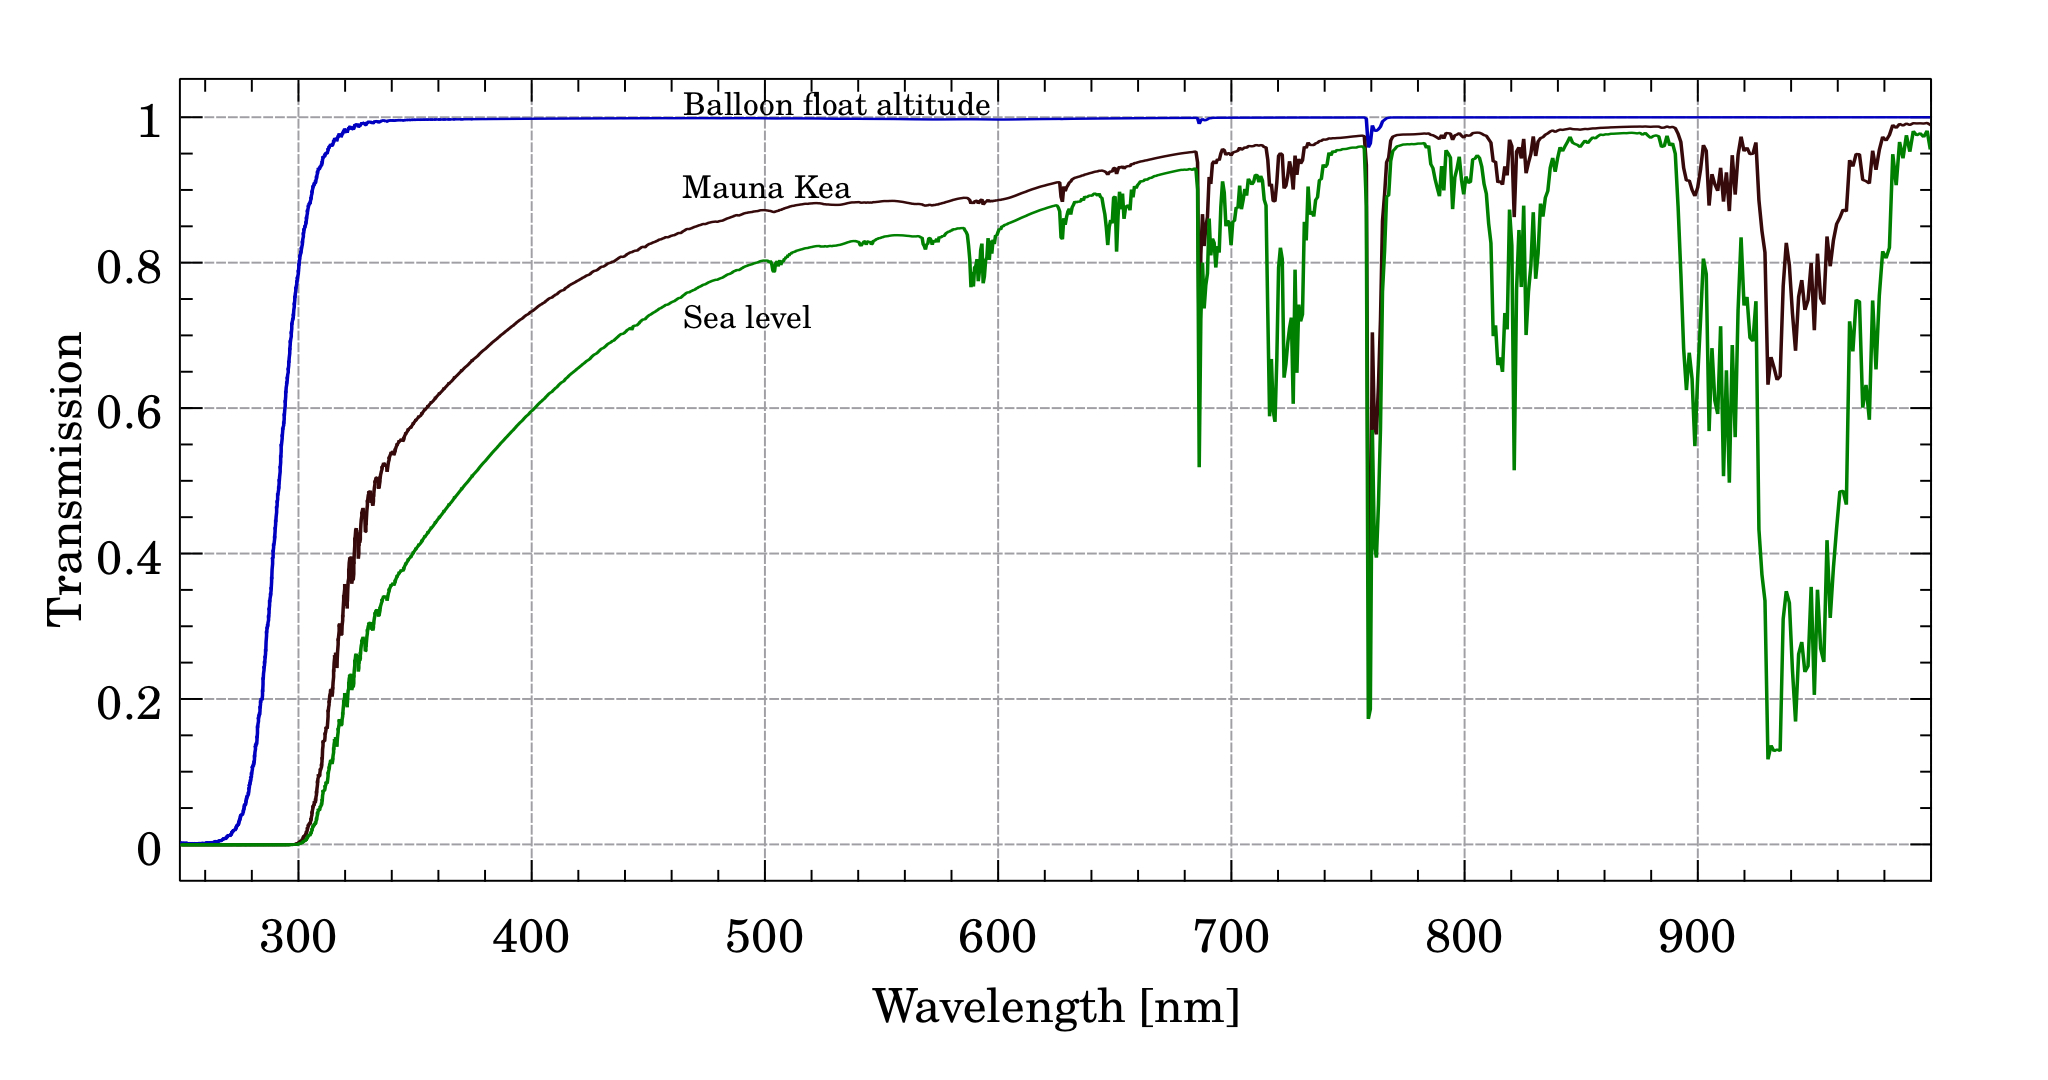
\includegraphics[width=0.95\textwidth]{Introduction/figs/atmosphere.jpg}
        \end{center}
        \caption{Transmission of the atmosphere vs wavelength at sea level (green), Mauna Kea (brown), and balloon float altitude (blue). }
        \label{fig:atmos}
    \end{small}
\end{figure}


\section{Super-pressure Balloon-borne Imaging Telescope (SuperBIT)}
SuperBIT provides near diffraction limited wide-field imaging from the stratosphere in the near UV and optical frequency range.  

The point of super bit is t be able to provide diffraction limited observations in the near uv and optical. The diffraction limit of the bit science camera is 0.25 arcseconds resolution therefore the stability of the system must be 2 order mags less which leaves us with a goal of 20 milliarcsecond stability this is achieved using two systems. first the gondola which gives a stability of 0.7" and then fgs in the optics that provides further stabilization by tip tilt the 100 marcsecond. Both systems described in more detail below.

\begin{figure}
    \begin{small}
        \begin{center}
            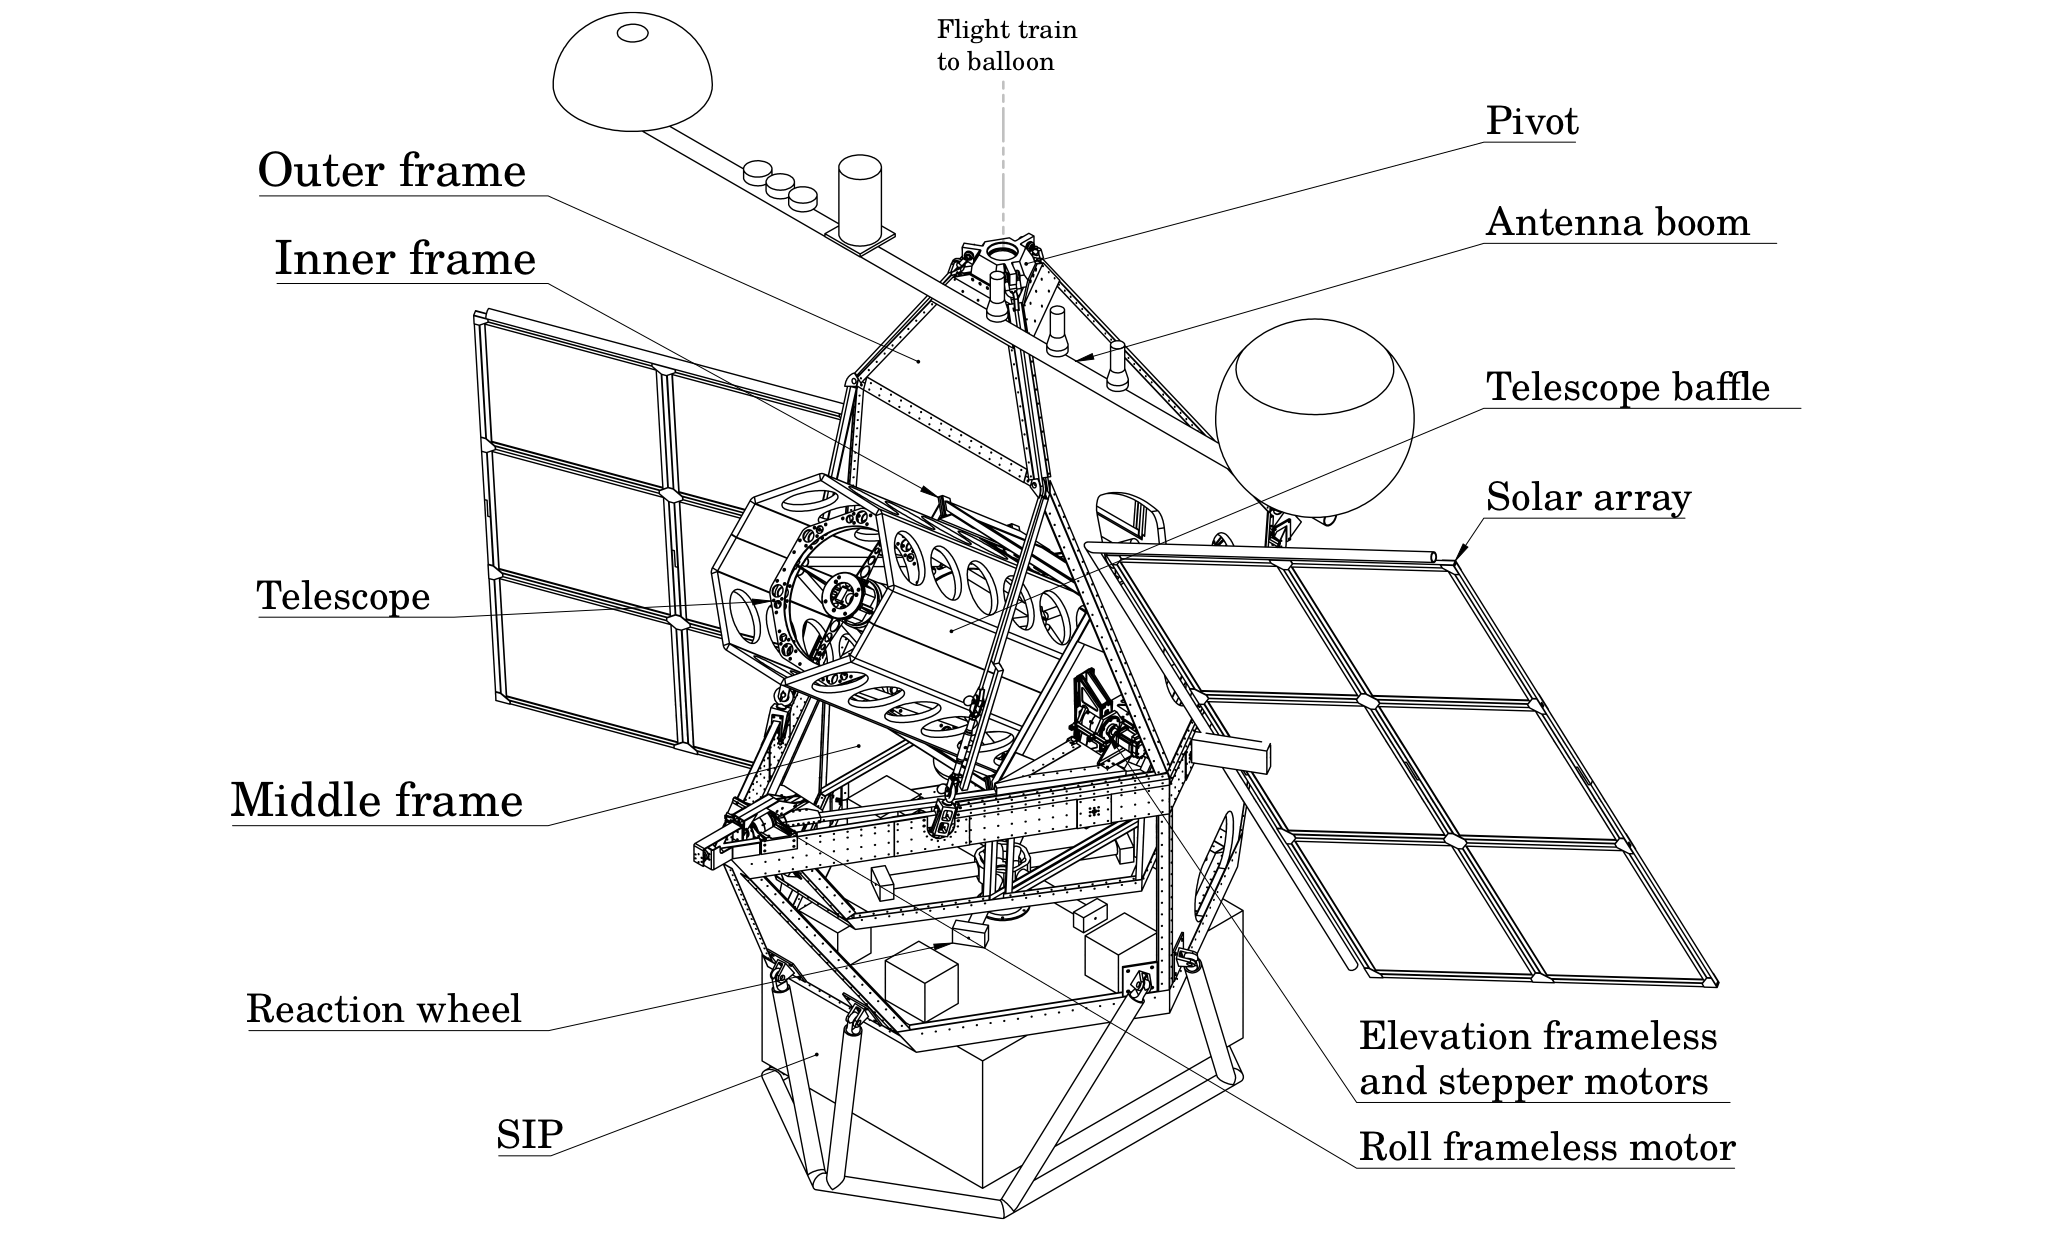
\includegraphics[width=0.95\textwidth]{Introduction/figs/bit_model.png}
        \end{center}
        \caption{Layout of the SuperBIT instrument.}
        \label{fig:bit}
    \end{small}
\end{figure}



\begin{figure}
    \begin{small}
        \begin{center}
            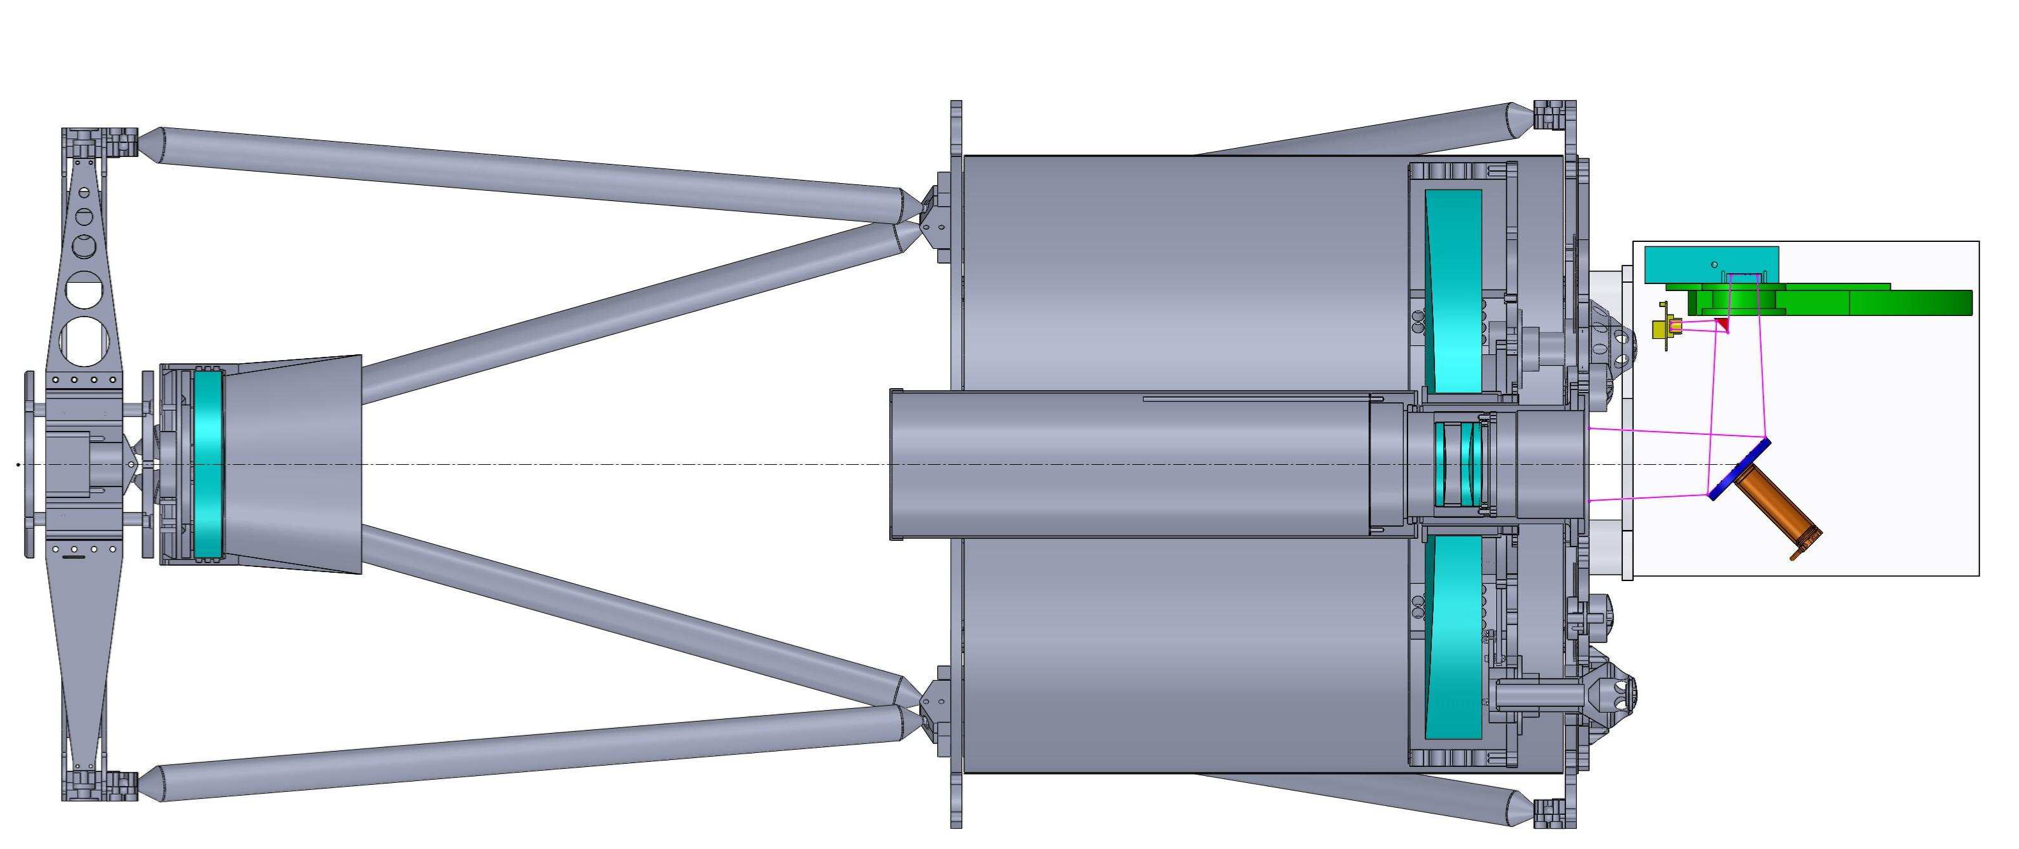
\includegraphics[width=0.95\textwidth]{Introduction/figs/optical_path.png}
        \end{center}
        \caption{The optical layout; The optical path (violet lines) is fed into the fine guidance system through the telescope (grey). The Tip/Tilt mirror (gold and blue) redirects the optical axis 90 degrees to the Science camera (cyan) through a filter wheel (green). Just before the filter wheel some of the light is redirected again by the pick-off mirror (red) to a star camera (yellow).}
        \label{fig:optics}
    \end{small}
\end{figure}

\par
For a more detailed description of the instrument please consult group alumni theses. For details on the electrical distribution systems and
superBIT mechatronics please see John Hartley's PhD thesis, for the mechanical structure see Steven Li’s Engineering Masters Thesis, for a detailed discussion of the controls system and software see Javier Romualdez’s PhD Thesis, for a detailed look at the star cameras system see Matthew Galloway’s PhD Thesis, and for details of the thermal control system see Susan Redmond’s Engineering Masters Theses.

